% This file was created with tikzplotlib v0.10.1.
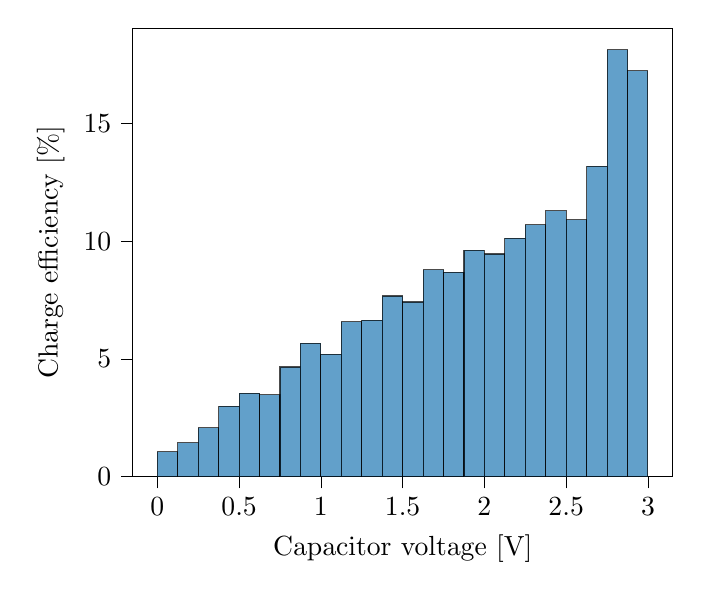
\begin{tikzpicture}

\definecolor{darkgray176}{RGB}{176,176,176}
\definecolor{steelblue31119180}{RGB}{31,119,180}

\begin{axis}[
tick align=outside,
tick pos=left,
x grid style={darkgray176},
xlabel={Capacitor voltage [V]},
xmin=-0.15, xmax=3.15,
xtick style={color=black},
y grid style={darkgray176},
ylabel={Charge efficiency [\%]},
ymin=0, ymax=19.0427020784769,
ytick style={color=black}
]
\draw[draw=black,fill=steelblue31119180,opacity=0.7] (axis cs:0,0) rectangle (axis cs:0.125,1.05844269421646);
\draw[draw=black,fill=steelblue31119180,opacity=0.7] (axis cs:0.125,0) rectangle (axis cs:0.25,1.43036599563255);
\draw[draw=black,fill=steelblue31119180,opacity=0.7] (axis cs:0.25,0) rectangle (axis cs:0.375,2.07965091405922);
\draw[draw=black,fill=steelblue31119180,opacity=0.7] (axis cs:0.375,0) rectangle (axis cs:0.5,2.99297080316369);
\draw[draw=black,fill=steelblue31119180,opacity=0.7] (axis cs:0.5,0) rectangle (axis cs:0.625,3.54297219678052);
\draw[draw=black,fill=steelblue31119180,opacity=0.7] (axis cs:0.625,0) rectangle (axis cs:0.75,3.48450357155878);
\draw[draw=black,fill=steelblue31119180,opacity=0.7] (axis cs:0.75,0) rectangle (axis cs:0.875,4.65181077150528);
\draw[draw=black,fill=steelblue31119180,opacity=0.7] (axis cs:0.875,0) rectangle (axis cs:1,5.6670439990114);
\draw[draw=black,fill=steelblue31119180,opacity=0.7] (axis cs:1,0) rectangle (axis cs:1.125,5.19280088348691);
\draw[draw=black,fill=steelblue31119180,opacity=0.7] (axis cs:1.125,0) rectangle (axis cs:1.25,6.57053403686955);
\draw[draw=black,fill=steelblue31119180,opacity=0.7] (axis cs:1.25,0) rectangle (axis cs:1.375,6.64431326209388);
\draw[draw=black,fill=steelblue31119180,opacity=0.7] (axis cs:1.375,0) rectangle (axis cs:1.5,7.66880558940446);
\draw[draw=black,fill=steelblue31119180,opacity=0.7] (axis cs:1.5,0) rectangle (axis cs:1.625,7.41225846160567);
\draw[draw=black,fill=steelblue31119180,opacity=0.7] (axis cs:1.625,0) rectangle (axis cs:1.75,8.79292067420482);
\draw[draw=black,fill=steelblue31119180,opacity=0.7] (axis cs:1.75,0) rectangle (axis cs:1.875,8.67413858533236);
\draw[draw=black,fill=steelblue31119180,opacity=0.7] (axis cs:1.875,0) rectangle (axis cs:2,9.6186074752565);
\draw[draw=black,fill=steelblue31119180,opacity=0.7] (axis cs:2,0) rectangle (axis cs:2.125,9.45119668148473);
\draw[draw=black,fill=steelblue31119180,opacity=0.7] (axis cs:2.125,0) rectangle (axis cs:2.25,10.114720045333);
\draw[draw=black,fill=steelblue31119180,opacity=0.7] (axis cs:2.25,0) rectangle (axis cs:2.375,10.7041333759687);
\draw[draw=black,fill=steelblue31119180,opacity=0.7] (axis cs:2.375,0) rectangle (axis cs:2.5,11.2947590953603);
\draw[draw=black,fill=steelblue31119180,opacity=0.7] (axis cs:2.5,0) rectangle (axis cs:2.625,10.9034990808974);
\draw[draw=black,fill=steelblue31119180,opacity=0.7] (axis cs:2.625,0) rectangle (axis cs:2.75,13.1799501165875);
\draw[draw=black,fill=steelblue31119180,opacity=0.7] (axis cs:2.75,0) rectangle (axis cs:2.875,18.1359067414065);
\draw[draw=black,fill=steelblue31119180,opacity=0.7] (axis cs:2.875,0) rectangle (axis cs:3,17.2423927150809);
\end{axis}

\end{tikzpicture}
